%%
%% This is file `sample-sigchi.tex',
%% generated with the docstrip utility.
%%
%% The original source files were:
%%
%% samples.dtx  (with options: `sigchi')
%% 
%% IMPORTANT NOTICE:
%% 
%% For the copyright see the source file.
%% 
%% Any modified versions of this file must be renamed
%% with new filenames distinct from sample-sigchi.tex.
%% 
%% For distribution of the original source see the terms
%% for copying and modification in the file samples.dtx.
%% 
%% This generated file may be distributed as long as the
%% original source files, as listed above, are part of the
%% same distribution. (The sources need not necessarily be
%% in the same archive or directory.)
%%
%% The first command in your LaTeX source must be the \documentclass command.
\documentclass[sigchi]{acmart}

\usepackage{subfigure,epsfig,amsfonts}
\usepackage{natbib}
\usepackage{amsmath}
\usepackage{amssymb}
\usepackage{amsthm}
\usepackage{bbm}
\usepackage[ruled,linesnumbered]{algorithm2e}

\usepackage{xcolor}
\usepackage{tikz}
\usetikzlibrary{calc}

\theoremstyle{definition}
\newtheorem{definition}{Definition}[section] 

\theoremstyle{theorem}
\newtheorem{theorem}{Theorem}[section] 

\theoremstyle{corollary}
\newtheorem{corollary}{Corollary}[section] 

\theoremstyle{lemma}
\newtheorem{lemma}{Lemma}[section] 

\theoremstyle{remark}
\newtheorem*{remark}{Remark}

\theoremstyle{prop}
\newtheorem{prop}{Proposition}[section] 

%%
%% \BibTeX command to typeset BibTeX logo in the docs
\AtBeginDocument{%
  \providecommand\BibTeX{{%
    \normalfont B\kern-0.5em{\scshape i\kern-0.25em b}\kern-0.8em\TeX}}}

%% Rights management information.  This information is sent to you
%% when you complete the rights form.  These commands have SAMPLE
%% values in them; it is your responsibility as an author to replace
%% the commands and values with those provided to you when you
%% complete the rights form.

\setcopyright{acmcopyright}
\copyrightyear{2019}
\acmYear{2019}

%% These commands are for a PROCEEDINGS abstract or paper.
\acmConference[Anchorage '19]{Anchorage '19: 15th International Workshop on Mining and Learning with Graphs}{August 05, 2019}{Anchorage, AK}
\acmBooktitle{Anchorage '19: 15th International Workshop on Mining and Learning with Graphs, August 05, 2019, Anchorage, AK}
\acmPrice{yy.yy}

%%
%% Submission ID.
%% Use this when submitting an article to a sponsored event. You'll
%% receive a unique submission ID from the organizers
%% of the event, and this ID should be used as the parameter to this command.
%%\acmSubmissionID{123-A56-BU3}

%%
%% The majority of ACM publications use numbered citations and
%% references.  The command \citestyle{authoryear} switches to the
%% "author year" style.
%%
%% If you are preparing content for an event
%% sponsored by ACM SIGGRAPH, you must use the "author year" style of
%% citations and references.
%% Uncommenting
%% the next command will enable that style.
%%\citestyle{acmauthoryear}

%%
%% end of the preamble, start of the body of the document source.
\begin{document}

%%
%% The "title" command has an optional parameter,
%% allowing the author to define a "short title" to be used in page headers.
\title{Covariant Compositional Networks for Learning Graphs}

%%
%% The "author" command and its associated commands are used to define
%% the authors and their affiliations.
%% Of note is the shared affiliation of the first two authors, and the
%% "authornote" and "authornotemark" commands
%% used to denote shared contribution to the research.

\author{Truong Son Hy}
\affiliation{
  \institution{University of Chicago}
  \city{Chicago, IL}
  \country{USA}
}
\email{hytruongson@uchicago.edu}

\author{Shubhendu Trivedi}
\affiliation{
  \institution{Toyota Technological Institute at Chicago}
  \city{Chicago, IL}
  \country{USA}
}
\email{shubhendu@uchicago.edu}

\author{Horace Pan}
\affiliation{
  \institution{University of Chicago}
  \city{Chicago, IL}
  \country{USA}
}
\email{hopan@uchicago.edu}

\author{Brandon M. Anderson}
\affiliation{
  \institution{University of Chicago}
  \city{Chicago, IL}
  \country{USA}
}
\email{brandona@uchicago.edu}

\author{Risi Kondor}
\affiliation{
  \institution{University of Chicago}
  \city{Chicago, IL}
  \country{USA}
}
\email{risi@uchicago.edu}

%%
%% By default, the full list of authors will be used in the page
%% headers. Often, this list is too long, and will overlap
%% other information printed in the page headers. This command allows
%% the author to define a more concise list
%% of authors' names for this purpose.
\renewcommand{\shortauthors}{Hy et. al}

%%
%% The abstract is a short summary of the work to be presented in the
%% article.
\begin{abstract}
In this paper, we propose Covariant Compositional Networks (CCNs), the state-of-the-art generalized convolution graph neural network for learning graphs. By applying higher-order representations and tensor contraction operations that are permutation-invariant with respect to the set of vertices, CCNs address the representation limitation of all existing neural networks for learning graphs in which permutation invariance is only obtained by summation of feature vectors coming from the neighbors for each vertex via well-known message passing scheme. \\ \\
For an application of learning small-scale molecular graphs, we investigate the efficiency of CCNs in estimating Density Functional Theory (DFT) that is the most successful and widely used approach to compute the electronic structure of matter but significantly expensive in computation. We obtain a very promising result and outperform other state-of-the-art graph learning models in Harvard Clean Energy Project \cite{HCEP} and QM9 \cite{QM9} molecular datasets. %\\ \\
%We also apply CCNs to learn large-scale networks such as Cora \& Citeseer \cite{Cora-Citeseer} in the task of semi-supervised transductive node classification. In addition, we combine CCNs with a scheme of hierarchical pooling to obtain a coarse-grained model that both increases robustness as well as computational saving.
\end{abstract}

%%
%% Keywords. The author(s) should pick words that accurately describe
%% the work being presented. Separate the keywords with commas.
\keywords{graph neural networks, graph learning, quantum chemistry, network analysis}


%%
%% This command processes the author and affiliation and title
%% information and builds the first part of the formatted document.
\maketitle

\section{Introduction}

In the field of Machine Learning, standard objects such as vectors, matrices, tensors were carefully studied and successfully applied into various areas including Computer Vision, Natural Language Processing, Speech Recognition, etc. However, none of these standard objects are efficient in capturing the structures of molecules, social networks or the World Wide Web which are not fixed in size. This arises the need of graph representation and extensions of Support Vector Machine and Convolution Neural Network to graphs. \\ \\
To represent graphs in general and molecules specifically, the proposed models must be \textit{permutation-invariant} and \textit{rotation-invariant}. In addition, to apply kernel methods on graphs, the proposed kernels must be \textit{positive semi-definite}. Many graph kernels and graph similarity functions have been introduced by researchers. Among them, one of the most successful and efficient is the Weisfeiler-Lehman graph kernel which aims to build a multi-level, hierarchical representation of a graph \citep{Shervashidze2011}. However, a limitation of kernel methods is quadratic space usage and quadratic time-complexity in the number of examples. The common idea of family of Weisfeiler-Lehman graph kernel is hashing the sub-structures of a graph. Extending this idea, we come to the simplest form of graph neural networks in which the \textit{fixed} hashing function is replaced by a \textit{learnable} one as a non-linearity mapping. In the context of graphs, the sub-structures can be considered as a set of vertex feature vectors. We ultilize the convolution operation by introducing higher-order representations for each vertex, from zeroth-order as a vector to the first-order as a matrix and the second-order as a 3rd order tensor. Also we introduce the notions of tensor contractions and tensor products to keep the orders of tensors manageable without exponentially growing. Our generalized convolution graph neural network is named as Covariant Compositional Networks (CCNs) \citep{Kondor2018, Hy2018}. We propose 2 specific algorithms that are first-order CCN in section \ref{section:ccn1d} and second-order CCN in section \ref{section:ccn2d}. 

\section{Compositional Networks}

In this section, we introduce a general architecture called \textbf{compositional networks} (\textbf{comp-nets}) for representing complex objects as a combination of their parts and show that graph neural networks can be seen as special cases of this framework.
\begin{definition}
Let $\mathcal{G}$ be an object with $n$ elementary parts (atoms) $\mathcal{E} = \{e_1, .., e_n\}$. A \textbf{compositional scheme} for $\mathcal{G}$ is a directed acyclic graph (DAG) $\mathcal{M}$ in which each node $\nu$ is associated with some subset $\mathcal{P}_{\nu}$ of $\mathcal{E}$ (these subsets are called \textbf{parts} of $\mathcal{G}$) in such a way that:
\begin{enumerate}
\item In the bottom level, there are exactly $n$ leaf nodes in which each leaf node $\nu$ is associated with an elementary atom $e$. Then $\mathcal{P}_\nu$ contains a single atom $e$.
\item $\mathcal{M}$ has a unique root node $\nu_r$ that corresponds to the entire set $\{e_1, .., e_n\}$.
\item For any two nodes $\nu$ and $\nu'$, if $\nu$ is a descendant of $\nu'$, then $\mathcal{P}_\nu$ is a subset of $\mathcal{P}_{\nu'}$. 
\end{enumerate}
\end{definition}
One can express message passing neural networks in this compositional framework. Consider a graph $G = (V, E)$ in an $L + 1$ layer network. The set of vertices $V$ is also the set of elementary atoms $\mathcal{E}$. Each layer of the graph neural network (except the last) has one node denoted by $\nu$ and one feature tensor denoted by $f$ for each vertex of the graph $G$. The compositional network $\mathcal{N}$ is constructed as follows:
\begin{enumerate}
\item In layer $\ell = 0$, each leaf node $\nu_i^0$ represents the single vertex $\mathcal{P}_i^0 = \{i\}$ for $i \in V$. The corresponding feature tensor $f_i^0$ is initialized by the vertex label $l_i$.
\item In layers $\ell = 1, 2, .., L$, node $\nu_i^\ell$ is connected to all nodes from the previous level that are neighbors of $i$ in $G$. The children of $\nu_i^\ell$ are $\{\nu_j^{\ell - 1}|j:(i, j) \in E\}$. Thus, $\mathcal{P}_i^\ell = \bigcup_{j:(i, j) \in E} \mathcal{P}_j^{\ell - 1}$. The feature tensor $f_i^\ell$ is computed as an aggregation of feature tensors in the previous layer:
$$f_i^\ell = \Phi(\{f_j^{\ell - 1}|j \in \mathcal{P}_i^\ell\})$$
where $\Phi$ is some aggregation function.
\item In layer $\ell = L + 1$, we have a single node $\nu_r$ that represents the entire graph and collects information from all nodes at level $\ell = L$:
$$\mathcal{P}_r \equiv V$$
$$f_r = \Phi(\{f_i^L|i \in \mathcal{P}_r\})$$
\end{enumerate}
In the following section, we will refer $\nu$ as the \textbf{neuron}, and $\mathcal{P}$ and $f$ as its corresponding \textbf{receptive field} and \textbf{activation}, respectively. 

\section{Covariance}

Standard message passing neural networks used summation or averaging operation as the aggregation function $\Phi$ of neighboring vertices' feature tensors. That would lead to loss of topological information. Therefore, we propose \textbf{permutation covariance} requirement for our neural activations $f$ defined as follows.
\begin{definition}
For a graph $G$ with the comp-net $\mathcal{N}$, and an isomorphic graph $G'$ with comp-net $\mathcal{N}'$, let $\nu$ be any neuron of $\mathcal{N}$ and $\nu'$ be the corresponding neuron of $\mathcal{N}'$. Assume that $\mathcal{P}_\nu = (e_{p_1}, .., e_{p_m})$ while $\mathcal{P}_{\nu'} = (e_{q_1}, .., e_{q_m})$, and let $\pi \in \mathbb{S}_m$ be the permutation that aligns the orderings of the two receptive fields, i.e., for which $e_{q_{\pi(a)}} = e_{p_a}$. We say that $\mathcal{N}$ is \textbf{covariant to permutations} if for any $\pi$, there is a corresponding function $R_\pi$ such that $f_{\nu'} = R_\pi(f_\nu)$.
\end{definition}
The definition can be understood as permuting the vertices of graph $G$ will change the activations of its vertices in a manner that is controlled by some fixed function $R_\pi$ that depends on the permuation $\pi$.

\section{First order Message Passing}
\label{section:ccn1d}

We will call the standard message passing as the \textbf{zero'th order message passing} in which each vertex is represented by a feature vector of length $c$ (or $c$ channels) which was not expressive enough to capture the structure of its local neighborhood. Hence, we propose \textbf{first order message passing} by representing each vertex $v$ by a matrix: $f_v^\ell \in \mathbb{R}^{|\mathcal{P}_v^\ell| \times c}$, each row of this feature matrix corresponds to a vertex in the neighborhood of $v$.
\begin{definition}
We say that $\nu$ is a \textbf{first order covariant node} in a comp-net if under the permutation of its receptive field $\mathcal{P}_\nu$ by any $\pi \in \mathbb{S}_{|\mathcal{P}_\nu|}$, its activation transforms as $f_\nu \mapsto P_\pi f_\nu$, where $P_\pi$ is the permutation matrix:
\begin{equation}
[P_\pi]_{i, j} \triangleq \begin{cases} 1, & \pi(j) = i  \\ 0, & otherwise \end{cases}
\end{equation}
The transformed activation $f_{\nu'}$ will be:
$$[f_{\nu'}]_{a, s} = [f_\nu]_{\pi^{-1}(a), s}$$
where $s$ is the channel index.
\end{definition}

\section{Second order Message Passing}
\label{section:ccn2d}

Instead of representing a vertex with a feature matrix as done in first order message passing, we can represent it by a 3rd order tensor $f_v^\ell \in \mathbb{R}^{|\mathcal{P}_v^\ell| \times |\mathcal{P}_v^\ell| \times c}$ and require these feature tensors to transform covariantly in a similar manner:
\begin{definition}
We say that $\nu$ is a \textbf{second order covariant node} in a comp-net if under the permutation of its receptive field $\mathcal{P}_\nu$ by an $\pi \in \mathbb{S}_{|\mathcal{P}_\nu|}$, its activation transforms as $f_\nu \mapsto P_\pi f_\nu P_\pi^T$. The transformed activation $f_{\nu'}$ will be:
$$[f_{\nu'}]_{a, b, s} = [f_\nu]_{\pi^{-1}(a), \pi^{-1}(b), s}$$
where $s$ is the channel index.
\end{definition}

\section{Third and higher order Message Passing}

The similar pattern is applied further for third, forth, and general, $k$'th order nodes in the comp-net, in which the activations are $k$'th order tensors, transforming under permutations as $f_\nu \mapsto f_{\nu'}$:
\begin{equation}
[f_{\nu'}]_{i_1, i_2, .., i_k, s} = [f_\nu]_{\pi^{-1}(i_1), \pi^{-1}(i_2), .., \pi^{-1}(i_k), s}
\label{eq:tensor-transform}
\end{equation}
All but the channel index $s$ (the last index) is permuted when we go from $f_\nu$ to $f_{\nu'}$ after some permutation $\pi$ of the receptive field $\mathcal{P}_\nu$. In general, we will call any quantiy which transforms according to this equation (ignoring the channel index) as a \textbf{k'th oder P-tensor}. Since scalars, vectors and matrices can be considered as zeroth, first and second order tensors, respectively, the following definition covers the previous definitions as special cases.
\begin{definition}
We say that $\nu$ is a \textbf{k'th order covariant node} in a comp-net if the corresponding activation $f_\nu$ is a k'th order P-tensor, i.e., it transforms under permutations of $\mathcal{P}_\nu$ according to \ref{eq:tensor-transform}. 
\end{definition}

\section{Tensor aggregation rules}
\label{section:tensor-rules}

The previous sections precribed how activations must transform in comp-nets of different orders. Tensor arithmetic provides a compact framework for deriving the general form of the permutation covariant operations. For convenience, we denote tensors as capital letters. Since the activation $f$ is a tensor in general, we will denote it by capital $F$ in the following sections. Recall the four basic operations that can be applied to tensors:
\begin{enumerate}
\item The \textbf{tensor product} of $A \in \mathcal{T}^k$ with $B \in \mathcal{T}^p$ yields a tensor $C = A \otimes B \in \mathcal{T}^{p + k}$ where:
$$C_{i_1, i_2, .., i_{k + p}} = A_{i_1, i_2, .., i_k} B_{i_{k + 1}, i_{k + 2}, .., i_{k + p}}$$
\item The \textbf{contraction} of $A \in \mathcal{T}^k$ along the pair of dimensions $\{a, b\}$ (assuming $a < b$) yields a $k - 2$ order tensor:
$$C_{i_1, i_2, .., i_k} = \sum\limits_j A_{i_1, .., i_{a - 1}, j, i_{a + 1}, .., i_{b - 1}, j, i_{b + 1}, .., k}$$
where we assume that $i_a$ and $i_b$ have been removed from the indices of $C$. Using Einstein notation, this can be written much more compactly as
$$C_{i_1, i_2, .., i_k} = A_{i_1, i_2, .., i_k} \delta^{i_a, i_b}$$
where $\delta^{i_a, i_b}$ is the diagonal tensor with $\delta^{i, j} = 1$ if $i = j$ and 0 otherwise. We also generalize contractions to (combinations of) larger sets of indices $\{\{a_1^1, .., a_{p_1}^1\}, \{a_1^2, .., a_{p_2}^2\}, .., \{a_1^q, .., a_{p_q}^q\}\}$ as the $(k - \sum_j p_j)$ order tensor:
$$C_{...} = A_{i_1, i_2, .., i_k} \delta^{a_1^1, .., a_{p_1}^1} \delta^{a_1^2, .., a_{p_2}^2} \cdot \cdot \cdot \delta^{a_1^q, .., a_{p_q}^q}$$
\item The \textbf{projection} of a tensor is defined as a special case of contraction:
$$A\downarrow_{a_1, .., a_p} = A_{i_1, i_2, .., i_k} \delta^{i_{a_1}} \delta^{i_{a_2}} \cdot \cdot \cdot \delta^{i_{a_k}}$$
where projection of $A$ among indices $a_1$, .., $a_p$ is denoted as $A\downarrow_{a_1, .., a_p}$.
\end{enumerate}
Proposition \ref{prop:combination} shows that all of the above operations as well as linear combinations preserve permutation covariance property of P-tensors. Therefore, they can be combined within the aggregation function $\Phi$.
\begin{prop}
Assume that $A$ and $B$ are $k$'th and $p$'th order P-tensors, respectively. Then:
\begin{enumerate}
\item $A \otimes B$ is a $(k + p)$'th order P-tensors.
\item $A_{i_1, i_2, .., i_k} \delta^{a_1^1, .., a_{p_1}^1} \cdot \cdot \cdot \delta^{a_1^q, .., a_{p_q}^q}$ is a $(k - \sum_j p_j)$'th order P-tensor.
\item If $A_1$, .., $A_u$ are $k$'th order P-tensors and $\alpha_1$, .., $\alpha_u$ are scalars, then $\sum_j \alpha_j A_j$ is a $k$'th order P-tensor.
\end{enumerate}
\label{prop:combination}
\end{prop}
Propositions \ref{prop:promotion}, \ref{prop:concatenation} and \ref{prop:production} show that tensor promotion, concatenation and production preverse permutation covariance, and hence can be applied within $\Phi$.
\begin{prop}
Assume that node $\nu$ is a descendant of node $\nu'$ in a comp-net $\mathcal{N}$. The corresponding receptive fields are $\mathcal{P}_\nu = (e_{p_1}, .., e_{p_m})$ and $\mathcal{P}_{\nu'} = (e_{q_1}, .., e_{q_{m'}})$. Remark that $\mathcal{P}_\nu \subseteq \mathcal{P}_{\nu'}$. Define $\chi^{\nu \rightarrow \nu'} \in \mathbb{R}^{m \times m'}$ as an indicator matrix:
\begin{equation}
\chi_{i, j}^{\nu \rightarrow \nu'} = \begin{cases} 1, & q_j = p_i \\ 0, & otherwise \end{cases}
\end{equation}
Assume that $F_\nu$ is a $k$'th order P-tensors with respect to permutations $(e_{p_1}, .., e_{p_m})$. We have the \textbf{promoted} tensor:
\begin{equation}
[F_{\nu \rightarrow \nu'}]_{i_1, .., i_k} = \chi_{i_1, j_1}^{\nu \rightarrow \nu'} \cdot \cdot \cdot \chi_{i_k, j_k}^{\nu \rightarrow \nu'} [F_\nu]_{j_1, .., j_k}
\label{eq:promotion}
\end{equation} 
is a $k$'th oder P-tensor with respect to permutations of $(e_{q_1}, .., e_{q_{m'}})$.
\label{prop:promotion}
\end{prop}
In equation \ref{eq:promotion}, node $\nu'$ promotes P-tensors from its children nodes $\nu$ with respect to its own receptive field $\mathcal{P}_{\nu'}$ by the appropriate $\chi^{\nu \rightarrow \nu'}$ matrix such that all promoted tensors $F_{\nu \rightarrow \nu'}$ have the same size. Remark that promoted tensors are padded with zeros.
\begin{prop}
Let nodes $\nu_1$, .., $\nu_n$ be the children of $\nu$ in a message passing type comp-net (the corresponding vertices of these nodes are in $\mathcal{P}_\nu$) with corresponding $k$'th order tensor activations $F_{\nu_1}$, .., $F_{\nu_n}$. Let
$$[F_{\nu_t \rightarrow \nu}]_{i_1, .., i_k} = [\chi^{\nu_t \rightarrow \nu}]_{i_1, j_1} \cdot \cdot \cdot [\chi^{\nu_t \rightarrow \nu}]_{i_k, j_k} [F_{\nu_t}]_{j_1, .., j_k}$$
be the promoted tensors ($t \in \{1, .., n\}$). We \textbf{concatenate} or \textbf{stack} them into a $(k + 1)$'th order tensor:
$$[\overline{F}_\nu]_{t, i_1, .., i_k} = [F_{\nu_t \rightarrow \nu}]_{i_1, .., i_k}$$
Then the concatenated tensor $\overline{F}_\nu$ is a $(k + 1)$'th order P-tensor of $\nu$.
\label{prop:concatenation}
\end{prop}
The restriction of the adjacency matrix to $\mathcal{P}_\nu$ is a second order P-tensor. Proposition \ref{prop:production} gives us a way to explicitly add topolocical information to the activation.
\begin{prop}
If $F_\nu$ is a $k$'th order P-tensor at node $\nu$, and $A\downarrow_{\mathcal{P}_\nu}$ is the restriction of the adjacency matrix to $\mathcal{P}_\nu$, then $F_\nu \otimes A\downarrow_{\mathcal{P}_\nu}$ is a $(k + 2)$'th order P-tensor.
\label{prop:production}
\end{prop}

\section{Second order tensor aggregation with the adjacency matrix}
\label{section:second_order_adjacency}

The first nontrivial tensor contraction case occurs when $F_{\nu_1 \rightarrow \nu}$, .., $F_{\nu_n \rightarrow \nu}$ are second order tensors, and we multiply with $A\downarrow_{\mathcal{P}_\nu}$, since in that case $\mathcal{T}$ is 5th order (6th order if we consider the channel index), and can be contracted down to second order in the following ways:
\begin{enumerate}
\item The \textbf{1+1+1} case contracts $\mathcal{T}$ in the form $\mathcal{T}_{i_1, i_2, i_3, i_4, i_5} \delta^{i_{a_1}} \delta^{i_{a_2}} \delta^{i_{a_3}}$, i.e., it projects $\mathcal{T}$ down along 3 of its 5 dimensions. This can be done in ${5 \choose 3} = 10$ ways.
\item The \textbf{1+2} case contracts $\mathcal{T}$ in the form $\mathcal{T}_{i_1, i_2, i_3, i_4, i_5} \delta^{i_{a_1}} \delta^{i_{a_2}, i_{a_3}}$, i.e., it projects $\mathcal{T}$ along one dimension, and contracts it along two others. This can be done in $3{5 \choose 3} = 30$ ways.
\item The \textbf{3} case is a single 3-fold contraction $\mathcal{T}_{i_1, i_2, i_3, i_4, i_5} \delta^{i_{a_1}, i_{a_2}, i_{a_3}}$. This can be done in ${5 \choose 3} = 10$ ways.
\end{enumerate}
Totally, we have 50 different contractions that result in 50 times more channels. In practice, we only implement 18 contractions for efficiency.

\section{Architecture}
\label{section:Architecture}

In this section, we will describe how our compositional architecture is a generalization of previous works with an extension to higher-order representations. \\ \\
Recent works on graph neural networks \cite{Duvenaud2015,KipfWelling2017,LiZemel2015,Gilmer2017} can all be seen as instances of \textit{zeroth order message passing} where each vertex representation is a vector (1st order tensor) of $c$ channels in which each channel is represented by a scalar (zeroth order P-tensor). This results in the loss of certain structural information during the message aggregation, and the network loses the ability to learn topological information of the graph's multiscale structure. \\ \\
Our architecture represents generalized vertex representations with higher-order tensors which can retain this structural information. There is significant freedom in the choice of this tensor structure, and we now explore two examples, corresponding to the tensor structures, which we call ``first order CCN'' and ``second order CCN'', respectively. \\ \\
We start with an input graph $G = (V, E)$ and construct a network with $L + 1$ levels, indexed from $0$ (input level) to $L$ (top level). Initially, each vertex $v$ is associated with an input feature vector $l_v \in \mathbb{R}^c$ where $c$ denotes the number of channels. The receptive field of vertex $v$ at level $\ell$ is denoted by $\mathcal{P}_v^\ell$ and is defined recursively as follows:
\begin{equation}
\mathcal{P}_v^\ell \triangleq \begin{cases} \{v\}, & \ell = 0 \\ \bigcup\limits_{(u, v) \in E} \mathcal{P}_u^\ell, & \ell = 1, \ldots, L \end{cases}
\end{equation}
The vertex representation of vertex $v$ at level $\ell$ is denoted by a feature tensor $F_v^\ell$. In zeroth order message passing, $F_v^{\ell} \in \mathbb{R}^c$ is a vector of $c$
channels. Let $N$ be the number of vertices in $\mathcal{P}_v^\ell$. In the first order CCN, each vertex is represented by a matrix (second order tensor) $F_v^\ell \in \mathbb{R}^{N \times c}$ in which each row corresponds to a vertex in the receptive field $\mathcal{P}_v^\ell$, and each channel is represented by a vector (first order P-tensor) of size $N$. In the second order CCN, $F_\ell^v$ is promoted into a third order tensor of size $N \times N \times c$ in which each channel has a second order representation (second order P-tensor). In general, we can imagine a series of feature tensors of increasing order for higher order message passing. Note that the components corresponding to the channel index does not transform as a tensor, whereas the remaining indices do transform as a P-tensor. The tensor $F_v^\ell$ transforms in a \textit{covariant} way with respect to the permutation of the vertices in the receptive field $\mathcal{P}_v^\ell$. \\ \\
Now that we have established the structure of the high order representations of the vertices at each site, we turn to the task of constructing the aggregation function $\Phi$ from one level to another. The key to doing this in a way that preserves covariance is to ``promote-stack-reduce'' the tensors as one traverses the network at each level. \\ \\
We start with the promotion step. Recall that we want to accumulate information at higher levels based upon the receptive field of a given vertex. However, it is clear that not all vertices in the receptive field have the same size tensors. To account for this, we use an index function $\chi$ that ensures all tensors are the same size by padding with zeros when necessary. At level $\ell$, given two vertices $v$ and $w$ such that $\mathcal{P}_w^{\ell - 1} \subseteq \mathcal{P}_v^\ell$, the permutation matrix $\chi_{\ell}^{w \rightarrow v}$ of size $|\mathcal{P}_v^\ell| \times |\mathcal{P}_w^{\ell - 1}|$ is defined as in Prop. \ref{prop:promotion}. In CCN 1D \& 2D, the resizing is done by (broadcast) matrix multiplication $\chi \cdot F_w^{\ell - 1}$ and $\chi \times F_w^{\ell - 1} \times \chi^T$ where $\chi = \chi_{\ell}^{w \rightarrow v}$, respectively. Denote the resized tensor as $F_{w \rightarrow v}^\ell$. (See step 7 in algorithm \ref{alg:second_order_algorithm}.) This promotion is done for all tensors of every vertex in the receptive field, and stacked/concatenated into a tensor one order higher. (See Prop. \ref{prop:concatenation}. Notice that the stacked index has the same size as the receptive field.) From here, as in CCN 2D, we can compute the \textit{tensor product} of this higher order tensor with the restricted adjacency matrix (subject to the receptive field) and obtain an even higher order tensor. (See Prop. \ref{prop:production}.) Finally, we can reduce the higher order tensor down to the expected size of the vertex representation using the tensor contractions discussed in Prop. \ref{prop:combination}. \\ \\
We include all possible tensor contractions, which introduces additional channels. To avoid an exponential explosion in the number of channels with deep networks, we use a learnable set of weights that reduces the number of channels to a fixed number $c$. These weights are learnable through backpropagation. To complete our construction of $\Phi$, this tensor is passed through an element-wise nonlinear function $\Upsilon$ such as a ReLU to form the feature tensor for a given vertex at the next level. (See steps 4 and 9 in algorithm \ref{alg:second_order_algorithm}.) \\ \\
Finally, at the output of the network, we again reduce the vertex representations $F_v^\ell$ into a vector of channels $\Theta(F_v^\ell) = F_v^\ell\downarrow_{i_1, .., i_p}$ where $i_1, .., i_p$ are the non-channel indices. (See Prop. \ref{prop:combination}.) We sum up all the reduced vertex representations of a graph to get a single vector which we use as the graph representation. This final graph representation can then be used for regression or classification with a fully connected layer. In addition, we can construct a richer graph representation by concatenating the shrunk representation at each level. (See steps 12, 13 and 14 in algorithm \ref{alg:second_order_algorithm}.) \\ \\
The development of higher order CCNs require efficient tensor algorithms to successively train the network. A fundamental roadblock we face in implementing CCNs is that fifth or sixth order tensors are often too large to be held in memory. To address this challenge, we do not construct the tensor product explicitly. Instead we introduce a \textit{virtual indexing system} for a \textit{virtual tensor} that computes the elements of tensor only when needed given the indices. This allows us to implement the tensor contraction operations efficiently with GPUs on virtual tensors. \\ \\
For example, consider the operations in step 8 in algorithm \ref{alg:second_order_algorithm}.  This requires performing contractions over several indices on the two inputs $\mathcal{F} = \{F_{w \rightarrow v}^\ell | w \in \mathcal{P}_v^\ell\}$, in which $\mathcal{F}_{i_1} = F_{w_{i_1} \rightarrow v}^\ell$ is of size $|\mathcal{P}_v^\ell| \times |\mathcal{P}_v^\ell| \times c$, and $\mathcal{A} = A\downarrow_{\mathcal{P}_v^\ell}$. One naive strategy would be to stack all tensors in $\mathcal{F}$ into a new object and then directly compute the tensor product with $\mathcal{A}$ to form a sixth order tensor, given by a tuple of indices $(i_1, i_2, i_3, i_4, i_5, i_6)$. Instead, the corresponding tensor element is computed on-the-fly through simple multiplication:
\begin{equation}
\mathcal{T}_{i_1, i_2, i_3, i_4, i_5, i_6} = (\mathcal{F}_{i_1})_{i_2, i_3, i_6} \cdot \mathcal{A}_{i_4, i_5}
\end{equation}
where $i_6$ is the channel index. \\ \\
In our experiments of CCN 2D, we implement 18 different contractions (see Prop. \ref{section:second_order_adjacency}) such that each contraction results in a $|\mathcal{P}_v^\ell| \times |\mathcal{P}_v^\ell| \times c$ tensor. The result of step 8 is $\overline{F}_\ell^v$ with 18 times more channels. \\ \\
Algorithm CCN 1D is described in pseudocode \ref{alg:first_order_algorithm}. Figure \ref{fig:first_order} shows a visualization of CCN 1D's tensors on C$_2$H$_4$ molecular graph. Vertices $e_3$ and $e_4$ are carbon (C) atoms, and vertices $e_1$, $e_2$, $e_5$ and $e_6$ are hydrogen (H) atoms. Edge $(e_3, e_4)$ is a double bond (C, C) between two carbon atoms. All other edges are single bonds (C, H) between a carbon atom and a hydrogen atom. In the bottom layer $\ell = 0$, the receptive field of every atom $e$ only contains itself, thus its representation $F_e^0$ is a tensor of size $1 \times c$ where $c$ is the number of channels (see figure \ref{fig:first_order}(a)). In the first layer $\ell = 1$, the receptive field of a hydrogen atom contains itself and the neighboring carbon atom (i.e., $\mathcal{P}_{e_1}^1 = \{e_1, e_3\}$), thus tensors for hydrogen atoms are of size $2 \times c$. Meanwhile, the receptive field of a carbon atom contains itself, the another carbon and two other neighboring hydrogens (i.e., $\mathcal{P}_{e_3}^1 = \{e_1, e_2, e_3, e_4\})$ and $\mathcal{P}_{e_4}^1 = \{e_3, e_4, e_5, e_6\}$), thus $F_{e_3}^1, F_{e_4}^1 \in \mathbb{R}^{4 \times c}$ (see figure \ref{fig:first_order}(b)). In all later layers denoted $\ell = \infty$, the receptive field of every atom contains the whole graph (in this case, 6 vertices in total), thus $F_e^\infty \in \mathbb{R}^{6 \times c}$ (see figure \ref{fig:first_order}(c)). \\ \\
\begin{figure}
\caption{\label{fig:first_order} CCN 1D on C$_2$H$_4$ molecular graph}
\centering
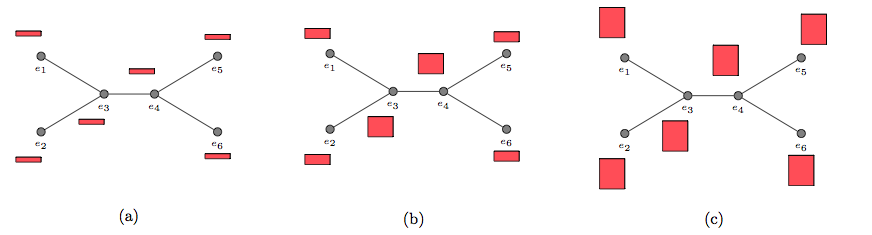
\includegraphics[scale=0.3]{first_order}
\end{figure}

\begin{algorithm}
{\bfseries Input:} $G$, $l_v$, $L$ \\
{\bfseries Parameters:} Matrices $W_0 \in \mathbb{R}^{c \times c}$, $W_1, .., W_L \in \mathbb{R}^{(2c) \times c}$ and biases $b_0, .., b_L$. For CCN 1D, we only implement 2 tensor contractions. \\
$F_v^0 \leftarrow \Upsilon(W_0 l_v + b_0 \mathbbm{1})$ $(\forall v \in V)$ \\
Reshape $F_v^0$ to $1 \times c$ $(\forall v \in V)$ \\
\For{$\ell = 1, .., L$}{
	\For{$v \in V$}{
		$F_{w \rightarrow v}^\ell \leftarrow \chi \times F_w^{\ell - 1}$ where $\chi = \chi_{w \rightarrow v}^\ell$ $(\forall w \in \mathcal{P}_v^\ell)$ \\
		Concatenate the promoted tensors in $\{F_{w \rightarrow v}^\ell | w \in \mathcal{P}_v^\ell\}$ and apply 2 tensor contractions that results in $\overline{F}_v^\ell \in \mathbb{R}^{|\mathcal{P}_v^\ell| \times (2c)}$. \\
		$F_v^\ell \leftarrow \Upsilon(\overline{F}_v^\ell \times W_\ell + b_\ell \mathbbm{1})$
	}
}
$F^\ell \leftarrow \sum_{v \in V} \Theta(F_v^\ell)$ $(\forall \ell)$ \\
Graph feature $F \leftarrow \bigoplus\limits_{\ell = 0}^L F^\ell \in \mathbb{R}^{(L + 1)c}$ \\
Use $F$ for downstream tasks.
\caption{\label{alg:first_order_algorithm} First-order CCN}
\end{algorithm}

Algorithm CCN 2D is described in pseudocode \ref{alg:second_order_algorithm}. Figure \ref{fig:second_order} shows a visualization of CCN 2D's tensors on C$_2$H$_4$ molecular graph. In the bottom layer $\ell = 0$, $|\mathcal{P}_e^0| = 1$ and $F_e^0 \in \mathbb{R}^{1 \times 1 \times c}$ for every atom $e$ (see figure \ref{fig:second_order}(a)). In the first layer $\ell = 1$, $|\mathcal{P}_e^1| = 2$ and $F_e^1 \in \mathbb{R}^{2 \times 2 \times c}$ for hydrogen atom $e \in \{e_1, e_2, e_5, e_6\}$, and for carbon atoms $|\mathcal{P}_{e_3}^1| = |\mathcal{P}_{e_4}^1| = 4$ and $F_{e_3}^1, F_{e_4}^1 \in \mathbb{R}^{4 \times 4 \times c}$ (see figure \ref{fig:second_order}(b)). In all other layers $\ell = \infty$, $\mathcal{P}_e^\infty \equiv V$ and $F_e^\infty \in \mathbb{R}^{6 \times 6 \times c}$ ($\forall e$) (see figure \ref{fig:second_order}(c)).
\begin{figure}
\caption{\label{fig:second_order} CCN 2D on C$_2$H$_4$ molecular graph}
\centering
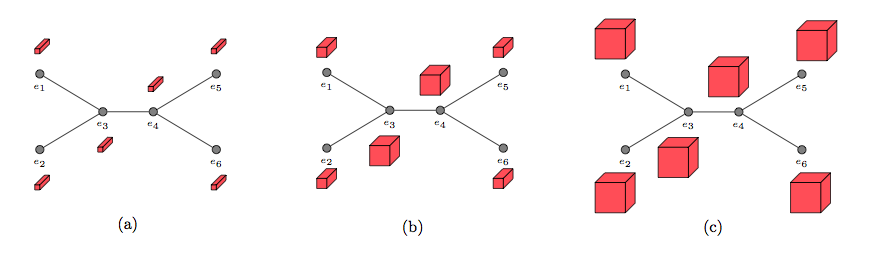
\includegraphics[scale=0.3]{second_order}
\end{figure}

\begin{algorithm}
{\bfseries Input:} $G$, $l_v$, $L$ \\
{\bfseries Parameters:} Matrices $W_0 \in \mathbb{R}^{c \times c}$, $W_1, .., W_L \in \mathbb{R}^{(18c) \times c}$ and biases $b_0, .., b_L$. \\
$F_v^0 \leftarrow \Upsilon(W_0 l_v + b_0 \mathbbm{1})$ $(\forall v \in V)$ \\
Reshape $F_v^0$ to $1 \times 1 \times c$ $(\forall v \in V)$ \\
\For{$\ell = 1, .., L$}{
	\For{$v \in V$}{
		$F_{w \rightarrow v}^\ell \leftarrow \chi \times F_w^{\ell - 1} \times \chi^T$ where $\chi = \chi_{w \rightarrow v}^\ell$ $(\forall w \in \mathcal{P}_v^\ell)$ \\
		Apply virtual tensor contraction algorithm (Sec.\ref{section:second_order_adjacency}) with inputs $\{F_{w \rightarrow v}^\ell | w \in \mathcal{P}_v^\ell\}$ and the restricted adjacency matrix $A\downarrow_{\mathcal{P}_v^\ell}$ to compute $\overline{F}_v^\ell \in \mathbb{R}^{|\mathcal{P}_v^\ell| \times |\mathcal{P}_v^\ell| \times (18c)}$. \\
		$F_v^\ell \leftarrow \Upsilon(\overline{F}_v^\ell \times W_\ell + b_\ell \mathbbm{1})$
	}
}
$F^\ell \leftarrow \sum_{v \in V} \Theta(F_v^\ell)$ $(\forall \ell)$ \\
Graph feature $F \leftarrow \bigoplus\limits_{\ell = 0}^L F^\ell \in \mathbb{R}^{(L + 1)c}$ \\
Use $F$ for downstream tasks.
\caption{\label{alg:second_order_algorithm} Second-order CCN}
\end{algorithm}

Figure \ref{fig:zero_to_second} shows the difference among zeroth, first and second order message passing (see from left to right) with layer $\ell \ge 2$. In the zeroth order, the vertex representation is always a vector of $c$ channels (see figure \ref{fig:zero_to_second}(a)). In the first and second order (see figures \ref{fig:zero_to_second}(b)(c)), the vertex representation is a matrix of size $6 \times c$ or a 3rd order tensor of size $6 \times 6 \times c$ in which each channels is represented by a vector of length $6$ or a matrix of size $6 \times 6$, respectively. With higher orders, CCNs can capture more topological information.
\begin{figure}
\caption{\label{fig:zero_to_second} Zeroth, first and second order message passing}
\centering
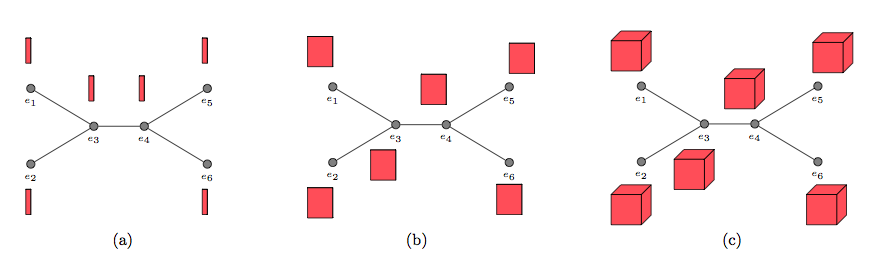
\includegraphics[scale=0.3]{zero_to_second}
\end{figure}

\section{Experiments}
\label{section:experiments}

We now compare our CCN framework (Section \ref{section:Architecture}) to several standard graph learning algorithms. We focus on two datasets that contain the result of a large number of Density Functional Theory (DFT) calculations:
\begin{enumerate}
\item \textbf{The Harvard Clean Energy Project (HCEP)}, consisting of 2.3 million organic compounds that are candidates for use in solar cells \citep{HCEP}. Figure \ref{fig:HCEP-example} shows an example of two molecules with similar graph structures in the HCEP dataset.
\item \textbf{QM9}, a dataset of $\sim$134k organic molecules with up to nine heavy atoms (C, O, N and F) \citep{QM9} out of the GDB-17 universe of molecules \citep{Ruddigkeit2012}. Each molecule contains data including 13 target chemical properties, along with the spatial position of every constituent atom.
\end{enumerate}
\begin{figure}
	\caption{\label{fig:HCEP-example} Molecules C$_{18}$H$_9$N$_3$OSSe (left) and C$_{22}$H$_{15}$NSeSi (right) with adjacency matrices}
	\centering
	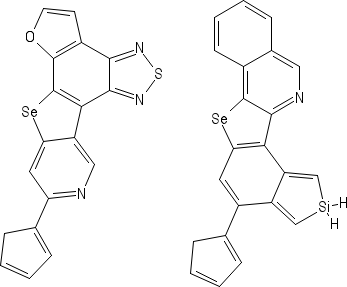
\includegraphics[scale=0.3]{sketcher2} \\
	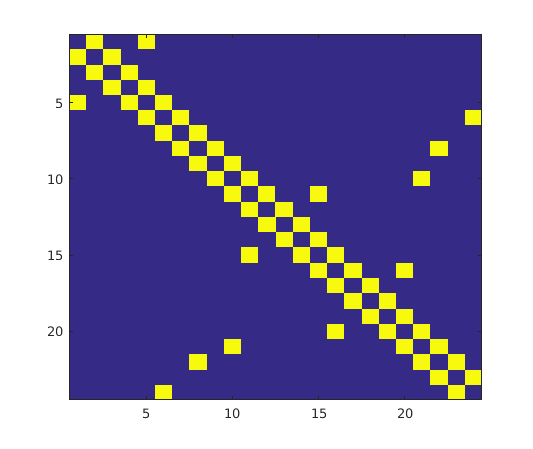
\includegraphics[scale=0.3]{adjacency1}
	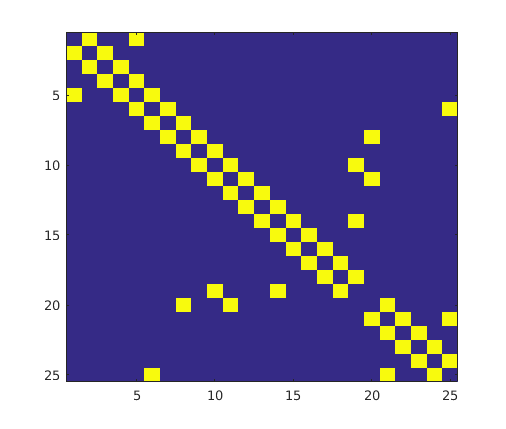
\includegraphics[scale=0.3]{adjacency2}
\end{figure}
DFT \citep{HohenbergKohn1964,KohnSham1965} is the workhorse of the molecular chemistry community, given its favorable tradeoff between accuracy and computational power. Still, it is too costly for tasks such as drug discovery or materials engineering, which may require searching through millions of candidate molecules. An accurate prediction of molecular properties would significantly aid in such tasks. \\ \\
We are interested in the ability of our algorithm to learn on both pure graphs, and also on physical data. As such, we perform three experiments. We start with two experiments based only upon atomic identity and molecular graph topology:
\begin{enumerate}
\item \textbf{HCEP}: We use a random sample of 50,000 molecules of the HCEP dataset; our learning target is Power Conversion Efficiency (PCE), and we present the mean average error (MAE). The input vertex feature $l_v$ is a one-hot vector of atomic identity concatenated with purely synthesized graph-based features.
\item \textbf{QM9(a)}: We predict the 13 target properties of every molecule. For this text we consider only heavy atoms and exclude hydrogen. Vertex feature initialization is performed in the same manner as the HCEP experiment. For training the neural networks, we normalized all 13 learning targets to have mean 0 and standard deviation 1. We report the MAE with respect to the normalized learning targets.
\end{enumerate}
We also tested our algorithm's ability to learn on DFT data based upon physical features. We perform the following experiment:
\begin{enumerate}
\setcounter{enumi}{2}
\item \textbf{QM9(b)}: The QM9 dataset with each molecule including hydrogen atoms. We use both physical atomic information (vertex features) and bond information (edge features) including: atom type, atomic number, acceptor, donor, aromatic, hybridization, number of hydrogens, Euclidean distance and Coulomb distance between pair of atoms. All the information is encoded in a vectorized format. \\ \\
To include the edge features into our model along with the vertex features, we used the concept of a \textit{line graph} from graph theory. We constructed the line graph for each molecular graph in such a way that: an edge of the molecular graph corresponds to a vertex in its line graph, and if two edges in the molecular graph share a common vertex then there is an edge between the two corresponding vertices in the line graph. (See Fig. \ref{fig:linegraph}). The edge features become vertex features in the line graph. The inputs of our model contain both the molecular graph and its line graph. The feature vectors $F_\ell$ between the two graphs are merged at each level $\ell$. (See step 12 of the algorithm \ref{alg:second_order_algorithm}). \\ \\
In QM9(b), we report the mean average error for each learning target in its corresponding physical unit and compare it against the Density Functional Theory (DFT) error given by \citep{Faber2017}. 
\end{enumerate}
In the case of HCEP, we compared CCNs to lasso, ridge regression, random forests, gradient boosted trees, optimal assignment Weisfeiler--Lehman graph kernel \citep{Kriege16} (WL), neural graph fingerprints \citep{Duvenaud2015}, and the ``patchy-SAN'' convolutional type algorithm (referred to as PSCN) \citep{Niepert2016}. For the first four of these baseline methods, we created simple feature vectors from each molecule: the number of bonds of each type (i.e., number of H--H bonds, number of C--O bonds, etc.) and the number of atoms of each type. Molecular graph fingerprints uses atom labels of each vertex as base features. For ridge regression and lasso, we cross validated over $\lambda$. For random forests and gradient boosted trees, we used 400 trees, and cross validated over max depth, minimum samples for a leaf, minimum samples to split a node, and learning rate (for GBT). For neural graph fingerprints, we used 3 layers and a hidden layer size of 10. In PSCN, we used a patch size of 10 with two convolutional layers and a dense layer on top as described in their paper. \\ \\
For QM9(a), we compared against the Weisfeiler--Lehman graph kernel, neural graph fingerprints, and PSCN. The settings for NGF and PSCN are as described for HCEP. For QM9(b), we compared against DFT error provided in \citep{Faber2017}. \\ \\
We initialized the synthesized graph-based features of each vertex with computed histogram alignment features, inspired by \citep{Kriege16}, of depth up to 10. Each vertex receives a base label $l_v= \text{concat}_{d = 1}^{10} {H_v^d}$ where $H_v^d \in \mathbb{R}^c$ (with $c$ being the total number of distinct discrete node labels) is the vector of relative frequencies of each label for the set of vertices at distance equal to $d$ from vertex $v$. Our CCNs architecture contains up to five levels. \\ \\
In each experiment we separated 80\% of the dataset for training, 10\% for validation, and evaluated on the remaining 10\% test set. We used Adam optimization \citep{Kingma2015} with the initial learning rate set to 0.001 after experimenting on a held out validation set. The learning rate decayed linearly after each step towards a minimum of $10^{-6}$. \\ \\
Our method, Covariant Compositional Networks, and other graph neural networks such as Neural Graph Fingerprints \citep{Duvenaud2015}, PSCN \citep{Niepert2016} and Gated Graph Neural Networks \citep{LiZemel2015} are implemented based on the GraphFlow framework (see chapter \ref{chapter:GraphFlow}). \\ \\
Tables \ref{tbl:hcep}, \ref{tbl:qm9mae}, and \ref{tbl:qm9mae-b} show the results of HCEP, QM9(a) and QM9(b) experiments, respectively. Figures \ref{fig:PCA-WL} and \ref{fig:PCA-CCN} show the 2D PCA projections of \textit{learned} molecular representations in HCEP dataset with Weisfeiler-Lehman, Covariant Compositional Networks 1D \& 2D, respectively. On the another hand, figures \ref{fig:tSNE-WL} and \ref{fig:tSNE-CCN} show the 2D projections with t-SNE \citep{Maaten2008}. The colors represent the PCE values ranging from 0 to 11. Figure \ref{fig:Result-CCN} shows the distributions between ground-truth and prediction of CCN 1D \& 2D in HCEP.
\begin{figure}
\caption{\label{fig:PCA-WL} 2D PCA projections of Weisfeiler-Lehman features in HCEP}
\centering
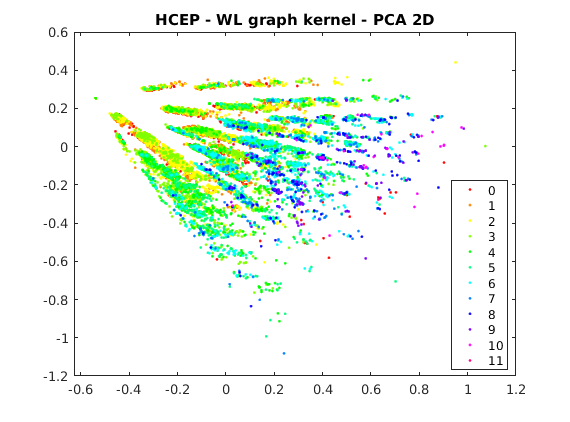
\includegraphics[scale=0.5]{PCA_WL}
\end{figure}
\begin{figure}
\caption{\label{fig:PCA-CCN} 2D PCA projections of CCNs graph representations in HCEP}
\centering
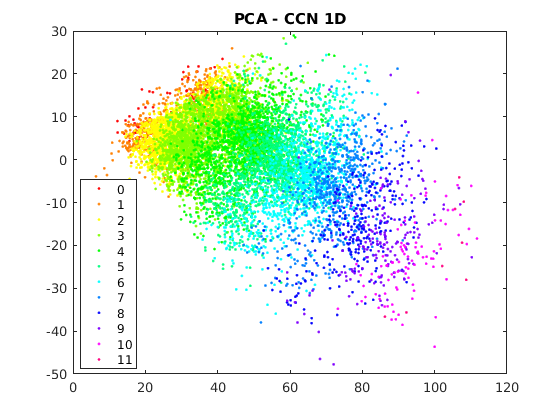
\includegraphics[scale=0.5]{PCA_CCN_1D}
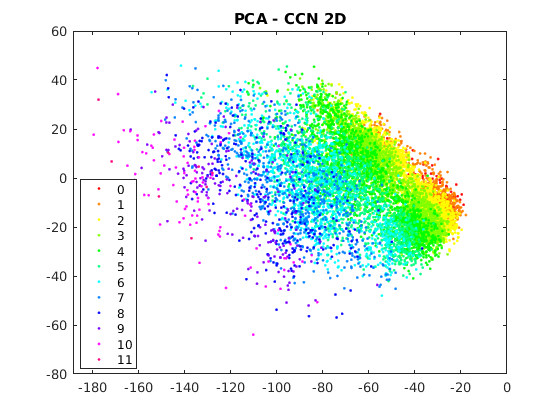
\includegraphics[scale=0.5]{PCA_CCN_2D}
\end{figure}
\begin{figure}
\caption{\label{fig:tSNE-WL} 2D t-SNE projections of Weisfeiler-Lehman features in HCEP}
\centering
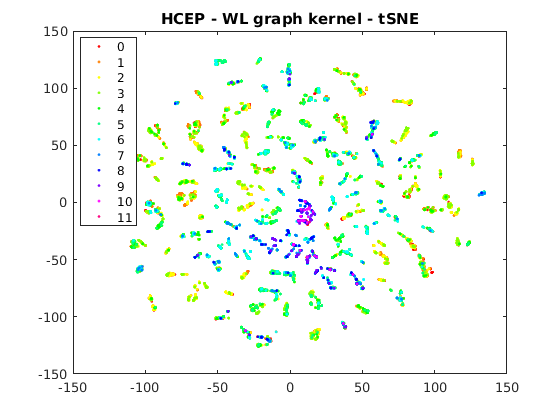
\includegraphics[scale=0.5]{tSNE_WL}
\end{figure}
\begin{figure}
\caption{\label{fig:tSNE-CCN} 2D t-SNE projections of CCNs graph representations in HCEP}
\centering
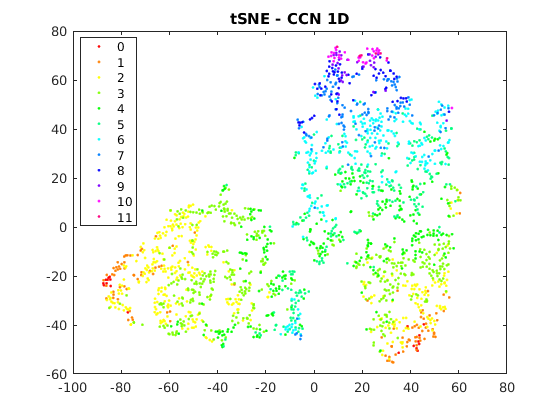
\includegraphics[scale=0.5]{tSNE_CCN_1D}
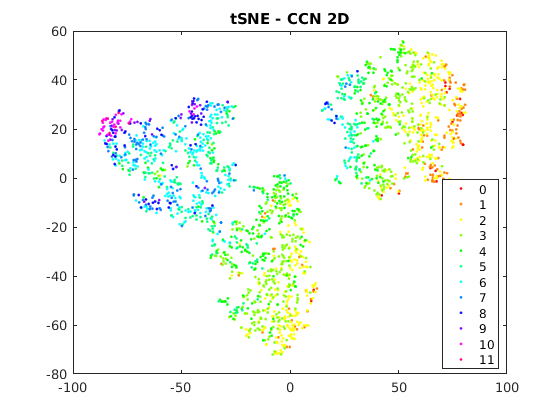
\includegraphics[scale=0.5]{tSNE_CCN_2D}
\end{figure}

\tikzset{
    vcircle/.style={
        circle, draw=black, minimum size=0.5em, inner sep=0pt, fill=gray
    },
    tensorfill/.style={
        fill=red!60, draw=black, text=black
    }
}

\begin{figure}[t]
\begin{center}
\begin{tikzpicture}

\node[vcircle, label={below: \tiny $e_1$}] (v1) at (-1.75, 0.75) {};
\node[vcircle, label={below: \tiny $e_2$}] (v2) at (-1.75, -0.75) {};
\node[vcircle, label={below: \tiny $e_3$}] (v3) at (-0.5, 0) {};
\node[vcircle, label={below: \tiny $e_4$}] (v4) at (0.5, 0) {};
\node[vcircle, label={below: \tiny $e_5$}] (v5) at (1.75, 0.75) {};
\node[vcircle, label={below: \tiny $e_6$}] (v6) at (1.75, -0.75) {};

\draw (v1) -- (v3) node [pos=0.5, label=above: {\tiny \color{blue}$(1)$}] {}
      (v2) -- (v3) node[pos=0.5, label=below:  {\tiny \color{blue}$(2)$}]{}
      (v3) -- (v4) node[pos=0.5, label=above:  {\tiny \color{blue}$(3)$}]{}
      (v5) -- (v4) node[pos=0.5, label=above:  {\tiny \color{blue}$(4)$}]{}
      (v6) -- (v4) node[pos=0.5, label=below:  {\tiny \color{blue}$(5)$}]{};

% \node [circle, label={}, opacity=0] (c) at ($(v4) + (0:5)$)  {};
\node[vcircle, label={below: {\tiny \color{blue}$(3)$}}] (p3) at ($(v4) + (0: 4)$) {};
\node[vcircle, label={above: {\tiny \color{blue}$(4)$}}] (p4) at ($(p3) + (30: 1)$) {};
\node[vcircle, label={above: {\tiny \color{blue}$(1)$}}] (p1) at ($(p3) + (150: 1)$) {};
\node[vcircle, label={below: {\tiny \color{blue}$(2)$}}] (p2) at ($(p3) + (-150: 1)$) {};
\node[vcircle, label={below: {\tiny \color{blue}$(5)$}}] (p5) at ($(p3) + (-30: 1)$) {};

\draw (p1) -- (p3)
    (p2) -- (p1)
    (p2) -- (p3)
    (p4) -- (p3)
    (p5) -- (p4)
    (p5) -- (p3);


\end{tikzpicture}
\end{center}
\caption{\label{fig:linegraph} Molecular graph of C$_2$H$_4$ (left) and its corresponding line graph (right).}
\end{figure}

\begin{table}[t]
\caption{\label{tbl:hcep} HCEP regression results}
\centering
\begin{tabular}{||l | c | c ||}
	\hline
	& Test MAE & Test RMSE \\
	\hline\hline
	Lasso & 0.867 & 1.437 \\
	\hline
	Ridge regression & 0.854 & 1.376 \\
	\hline
	Random forest & 1.004 & 1.799 \\
	\hline
	Gradient boosted trees & 0.704 & 1.005 \\
	\hline
	WL graph kernel & 0.805 & 1.096 \\
	\hline
	Neural graph fingerprints & 0.851 & 1.177 \\
	\hline
	PSCN & 0.718 & 0.973 \\
	\hline
	CCN 1D & \textbf{0.216} & \textbf{0.291} \\
	\hline
	CCN 2D & \textbf{0.340} & \textbf{0.449} \\
	\hline
\end{tabular}
\end{table}



\begin{table}
\caption{\label{tbl:qm9mae} QM9(a) regression results (MAE)}
\begin{center}
\begin{tabular}{|| c | c | c | c | c ||}
	\hline
	Target              & WLGK 		& NGF 	& PSCN  			&  CCN 2D   \\
	\hline\hline
	alpha               & 0.46		& 0.43	& 0.20  			& \textbf{0.16}	    \\
	\hline
	Cv	                & 0.59  	& 0.47	& 0.27  			& \textbf{0.23}	    \\
	\hline
	G 	                & 0.51		& 0.46	& 0.33  			& \textbf{0.29}	    \\
	\hline
	gap 	            & 0.72		& 0.67	& 0.60  			& \textbf{0.54}	    \\
	\hline
	H 	                & 0.52		& 0.47	& 0.34  			& \textbf{0.30}	    \\
	\hline
	HOMO 	            & 0.64		& 0.58	& 0.51 				& \textbf{0.39}      \\
	\hline
	LUMO 	            & 0.70		& 0.65	& 0.59  			& \textbf{0.53}	    \\
	\hline
	mu	 				& 0.69		& 0.63	& 0.54  			& \textbf{0.48}		\\
	\hline
	omega1 				& 0.72		& 0.63	& 0.57  			& \textbf{0.45}		\\
	\hline
	R2	 				& 0.55		& 0.49	& 0.22  			& \textbf{0.19}	    \\
	\hline
	U	 	            & 0.52		& 0.47	& 0.34  			& \textbf{0.29}      \\
	\hline
	U0	                & 0.52		& 0.47	& 0.34  			& \textbf{0.29}	    \\
	\hline
	ZPVE 	            & 0.57		& 0.51	& 0.43  			& \textbf{0.39}	    \\
	\hline
\end{tabular}
\end{center}
\end{table}

\begin{table}
\caption{\label{tbl:qm9mae-b} QM9(b) regression results (MAE)}
\begin{center}
\begin{tabular}{|| c | c | c | c | c ||}
	\hline
	Target              & CCNs				& DFT error		& Physical unit   \\
	\hline\hline
	alpha               & \textbf{0.19}		& 0.4  			& $\text{Bohr}^3$ \\
	\hline
	Cv	                & \textbf{0.06}    	& 0.34			& cal/mol/K \\
	\hline
	G 	                & \textbf{0.05}   	& 0.1			& eV	\\
	\hline
	gap 	            & \textbf{0.11}		& 1.2   		& eV	\\
	\hline
	H 	                & \textbf{0.05}		& 0.1			& eV  \\
	\hline
	HOMO 	            & \textbf{0.08}		& 2.0  			& eV \\
	\hline
	LUMO 	            & \textbf{0.07}		& 2.6			& eV \\
	\hline
	mu	 				& 0.43				& \textbf{0.1}	& Debye	\\
	\hline
	omega1 				& \textbf{2.54}		& 28			& $\text{cm}^{-1}$	\\
	\hline
	R2	 				& 5.03				& -				& $\text{Bohr}^2$ \\
	\hline
	U	 	            & \textbf{0.06}		& 0.1			& eV  \\
	\hline
	U0	                & \textbf{0.05}		& 0.1			& eV	\\
	\hline
	ZPVE 	            & \textbf{0.0043}	& 0.0097		& eV \\
	\hline
\end{tabular}
\end{center}
\end{table}


\begin{figure}
\caption{\label{fig:Result-CCN} Distributions of ground-truth and prediction of CCN 1D \& 2D in HCEP}
\centering
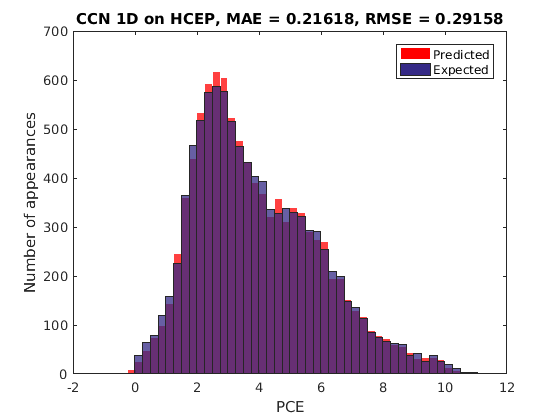
\includegraphics[scale=0.5]{Result_CCN_1D}
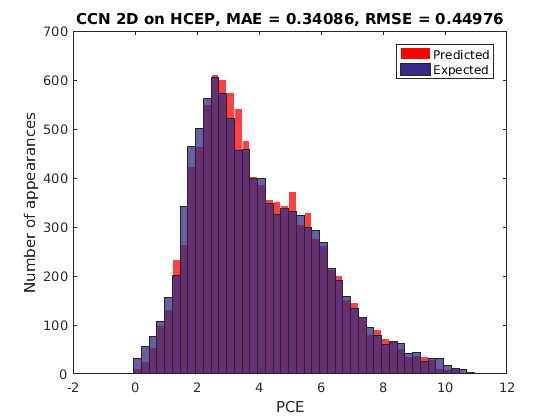
\includegraphics[scale=0.5]{Result_CCN_2D}
\end{figure}

\subsection{Discussion}
On the subsampled HCEP dataset, CCN outperforms all other methods by a very large margin. In the QM9(a) experiment, CCN obtains better results than three other graph learning algorithms for all 13 learning targets. In the QM9(b) experiment, our method gets smaller errors comparing to the DFT calculation in 11 out of 12 learning targets (we do not have the DFT error for R2).

\section{Conclusion}

We extended Message Passing Neural Networks and generalized convolution operation for Covariant Compositional Networks by higher-order representations in order to approximate Density Functional Theory. We obtained very promising results and outperformed other state-of-ther-art graph neural networks such as Neural Graph Fingerprint and Learning Convolutional Neural Networks on Harvard Clean Energy Project and QM9 datasets.

%%
%% The next two lines define the bibliography style to be used, and
%% the bibliography file.
\bibliographystyle{ACM-Reference-Format}
\bibliography{sample-base}

%%
%% If your work has an appendix, this is the place to put it.
\appendix


\end{document}
\endinput
%%
%% End of file `sample-sigchi.tex'.
